\documentclass[acmnow]{acmtrans2m}
\usepackage{amssymb}
\usepackage{amscd}
\usepackage{amsmath}
\usepackage[dvipdfm]{graphicx}
\usepackage{color}

\newtheorem{theorem}{Theorem}[section]
\newtheorem{conjecture}[theorem]{Conjecture}
\newtheorem{corollary}[theorem]{Corollary}
\newtheorem{proposition}[theorem]{Proposition}
\newtheorem{lemma}[theorem]{Lemma}
\newdef{definition}[theorem]{Definition}
\newdef{remark}[theorem]{Remark}

\def\F2{{\mathbb F}_2}
\def\wt{{\rm wt}}
\def\wo{{\rm wt}_o}
\def\wf{{\rm wt}_f}
\def\UL{{\rm ul}}
\def\bx{{{\mathbf x}}}
\def\by{{{\mathbf y}}}
\def\bz{{{\mathbf z}}}
\def\bw{{{\mathbf w}}}
\def\bu{{{\mathbf u}}}

\def\im{{\mathrm{Im}}}
\def\ker{{\mathrm{Ker}}}
\def\id{{\mathrm{Id}}}
\def\tr{{\mathrm{tr}}}

\title{SIMD-oriented Fast Mersenne Twister:
a 128-bit Pseudorandom Number Generator
}
            
\author{Mutsuo Saito and Makoto Matsumoto, Hiroshima University \\
}
            
\begin{abstract} 
Mersenne Twister (MT) 
is a widely used pseudorandom number generator (PRNG), 
which is fast and has a long period of $2^{19937}-1$.
On the other hand, recent CPUs for personal computers
has Single Instruction Multiple Data (SIMD) operations,
which are essentially 128-bit operations.  
In this paper, we shall propose a 128-bit based 
PRNG, which is analogous to MT but making full use
of SIMD operations, named SIMD-oriented Fast Mersenne Twister
(SFMT). The recursion of SFMT fits to the pipeline processing
better than MT, and SFMT is roughly twice faster than MT
that is optimized with SIMD operations.
Moreover, the dimension of equidistibution of SFMT, 
as a 32-bit integer generator,
is better than MT. 

We also introduce 
a block-generation function, 
which fills an array of 32-bit integers at one time,
which speeds up the generation by a factor of two. 
The speed comparison with other modern generators, 
such as multiplicative recursive generators,
shows big advantage of SFMT.
\end{abstract}
            
\category{G.3}{Mathematics of Computing}{PROBABILITY AND STATISTICS}[Random number generation]

\terms{Algorithms, Theory} 
            
\keywords{
Mersenne Twister,
SFMT, 
SIMD, 
128-bit,
block generation
}

\begin{document}
\maketitle

\begin{bottomstuff}
Authors' addresses: 
M. Saito and M. Matsumoto: Department of Mathematics, Hiroshima University,
Kagamiyama 1-3-1, Higashi-Hiroshima, Hiroshima 739-8526, Japan;
email: \{saito, m-mat\}@math.sci.hiroshima-u.ac.jp;

This study is partially supported by JSPS/Ministry of Education
Grant-in-Aid for Scientific Research No.18654021, No. 16204002,
and JSPS Core-to-Core Program No.18005.
\end{bottomstuff}

\section{Introduction}
Recently, the scale of simulations is getting larger,
and thus faster pseudorandom number generators (PRNG)
are required. In particular, the power of CPUs for
usual personal computers are now sufficiently strong,
and the necessity of efficient PRNGs is increasing.
One of such generators is Mersenne Twister (MT) \cite{MT}.
It is based on a linear recursion modulo 2, 
and a version MT19937 has the period of $2^{19937}-1$ and can generate
roughly $10^8$ 32-bit pseudorandom integers per a second.

On the other hand, modern CPUs for Personal Computers,
such as Pentium and Power PC, have 
Single Instruction Multiple Data (SIMD) operations,
which can be considered as operations 
on 128-bit registers. In addition, they have more registers
and automatic parallelisms by multi-stage pipelining. These features
are not reflected in the design of MT. 

In this article, we propose a MT-like 
pseudorandom number generator
that makes full use of these new features: SFMT, 
SIMD-oriented Mersenne Twister. 
We implemented an SFMT with period $2^{19937}-1$,
with better equidistribution property than MT. 
SFMT is much faster than MT, even without using SIMD instructions. 

There is an argument that the cpu-time consumed for 
function call to PRNG routine occupies large part of
the random number generation, and consequently 
it is not significant to improve the speed of PRNG 
(cf. \cite{XORSHIFT}).
This is not always the case: 
one can avoid the function calls by (1) inline-expansion
and/or (2) generation of an array of pseudorandom numbers
at one call. Actually some demanding users re-coded MT to avoid the 
function call, see the homepage of \cite{MT}. 
In this article, we introduce a block-generation scheme, which 
is much faster than using function calls.

\section{SIMD-oriented Fast Mersenne Twister}\label{sec:jump}

We propose the SIMD-oriented Fast Mersenne Twister (SFMT) 
pseudorandom number generator. It is a generator based
on a linear recursion over $\F2$. 
We identify
the set of bit $\{0,1\}$
with the two element field $\F2$.
A $w$-bit integers are identified with 
a horisontal vector in $\F2^{w}$, and 
$+$ denotes the sum as vectors (i.e., 
bit-wise exor), not as integers.
We consider three cases: $w$ is 32, 64 or 128.

\subsection{LFSR generators}
We generate
a sequence $\bx_0, \bx_1, \bx_2, \ldots$
of elements $\F2^{w}$ by a recursion
\begin{equation}\label{eq:recursion}
\bx_{i+N}:=g(\bx_i, \bx_{i+1}, \ldots, \bx_{i+N-1}),
\end{equation}
where $\bx_i \in \F2^{w}$ and 
$g:(\F2^{w})^N \to \F2^{w}$ is an $\F2$-linear function
(i.e., the multiplication of $(w \times wN)$-matrix)
and use it as a pseudorandom $w$-bit integer sequence.
This type of generator is called a Linear Feedbacked 
Shift Register (LFSR).

Mersenne Twister (MT) \cite{MT}
is an example with
$$
g(\bw_0,\ldots,\bw_{N-1})=(\bw_0|\bw_1)A + \bw_M,
$$
where $(\bw_0|\bw_1)$ denotes
the concatenation of 
$32-r$ MSBs of $\bw_0$ and $r$ LSBs of $\bw_1$,
and $A$ is a $(32\times 32)$-matrix 
for which $\bw A$ is computable 
by a few bit-operations.
Its period is $2^{32N-r}-1$, chosen to be a Mersenne prime.
To attain a better equidistribution property, 
MT transforms the sequence by
a suitably chosen $32\times 32$ matrix $T$, that is, 
the output sequence is 
$\bx_0T , \bx_1T, \bx_2T, \ldots$
(called tempering).

\subsection{New features of modern CPUs for personal computers.}
Modern CPUs for personal computers (e.g.\ Pentium and
PowerPC) have new features such as 
(1) integer multiplication instructions
(2) floating point operations 
(3) SIMD operations 
(4) multi-stage pipelining.
These were not available for standard CPUs for PC, when MT was designed.

An advantage of $\F2$-linear generators 
over integer multiplication generators 
(such as Linear Congruential Generators or Multiple
Recursive Generators \cite{MRG})
was the high-speed generation by avoiding multiplications.
This advantage is now smaller, since 
32-bit integer multiplication is quite fast. 

Among these features,
(3) and (4) fit to $\F2$-linear generators. 
Our simple idea is: to design
a 128-bit integer generator, considering
the benefit of such parallelism in the recursion.

\subsection{The recursion of SFMT}
We choose the recursion
\begin{eqnarray}\label{eq:rec-SFMT}
g(\bw_0,\ldots,\bw_{N-1}) 
%&=& g(\bw_0, \bw_M, \bw_{N-2}, \bw_{N-1}) \\
&=& \bw_0A + \bw_MB + \bw_{N-2}C + \bw_{N-1}D,
\end{eqnarray}
% \[x_{n+i} = x_{n-1+i}A + x_{n-2+i}B+ x_{m+i}C + x_{i}D,\]
where 
$\bw_0, \bw_M, \ldots$ are $w=$128-bit integers 
(= horisontal vectors in $\F2^{128}$),
and $A, B, C, D$ are sparse $128 \times 128$ matrices
for which 
$\bw A, \bw B, \bw C, \bw D$ can be computed by
a few SIMD bit-operations.
%\begin{figure}
%\begin{center}
%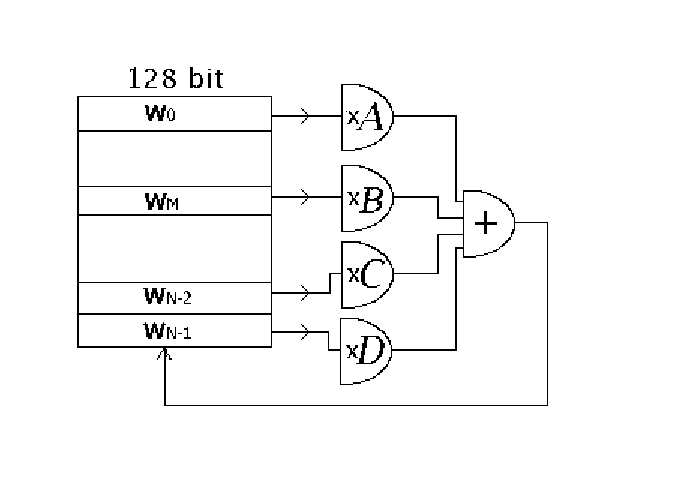
\includegraphics[width=0.7\linewidth]{sfmt-a.eps}
%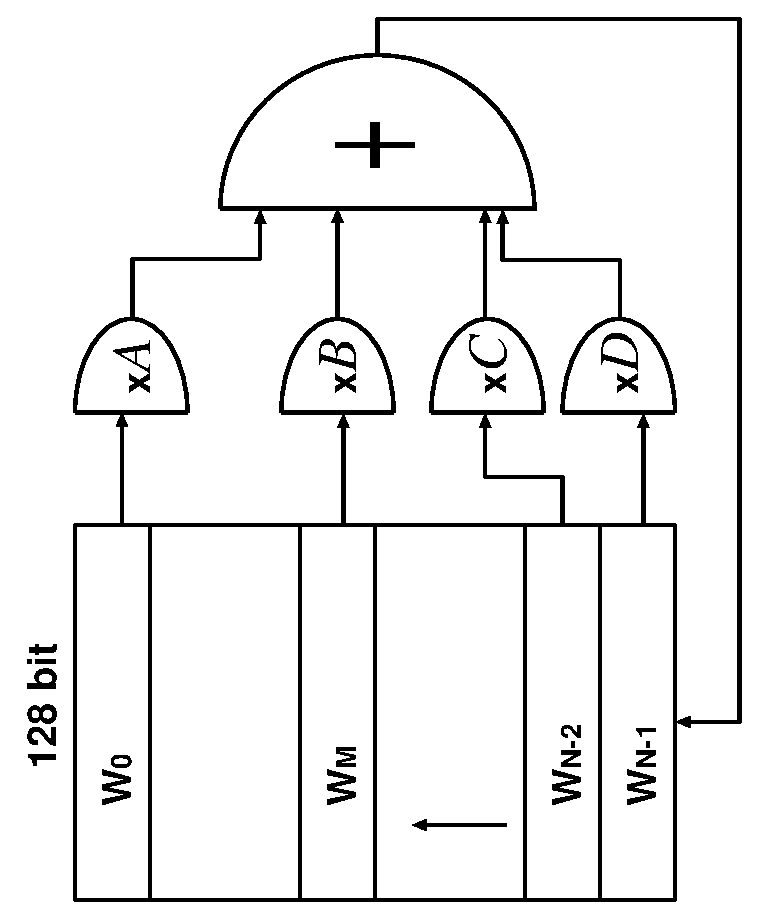
\includegraphics[width=0.7\linewidth]{sfmt-a2.eps}
%\end{center}
%\caption{The transition function of SIMD-oriented Fast MT.}
%\end{figure}
The choice of the suffixes $N-1$, $N-2$ is for the 
speed. In the computation of $g$, 
$\bw_0$ and $\bw_M$ are read from the memory array.
On the other hand, 
$\bw_{N-2}$ and $\bw_{N-1}$ are kept in two 128-bit
registers in the CPU, 
say {\tt r1} and {\tt r2}. We assign 
${\tt r2} \leftarrow {\tt r1}$ and
${\tt r1} \leftarrow \mbox{``the presently generated word''}$
at every generation.
The merit of doing this is to use pipeline effectively. To fetch 
$\bw_0$ and $\bw_M$ from the memory takes considerable
time. In the meanwhile, 
CPU can compute $\bw_{N-2}C$ and $\bw_{N-1}D$,
because $\bw_{N-2}$ and $\bw_{N-1}$ are kept 
in the registers.

By try-and-errors, 
we searched for a set of parameters of SFMT,
with period being a multiple of $2^{19937}-1$
and good equidistribution property.
The degree of recursion $N$ is $\lfloor 19937/128 \rfloor=156$, 
and the linear transformations $A,B,C,D$ are as follows.
\begin{itemize}
\item 
$\bw A := (\bw \stackrel{128}{<<} 8) + \bw.$

This notation means that $\bw$ is regarded
as a single 128-bit integer, and 
$\bw A$ is the result of the left-shift
of $\bw$ by 8 bits. There is such a SIMD operation
in both Pentium SSE2 and PowerPC altivec SIMD instruction 
sets (SSE2 permits only a multiple of 8
as the amount of shifting). 
Note that the notation $+$ means the exclusive-or
in this article.

\item
$\bw B := (\bw \stackrel{32}{>>} 11) \& \mbox{\tt BFFFFFF6 BFFAFFFF DDFECB7F DFFFFFEF}.$

This notation means that $\bw$ is considered to be 
a quadruple of $32$-bit integers, and
each $32$-bit integer is shifted to the right by 11 bit,
(thus the most significant bit is filled with a 0, 
for each 32-bit ingegers).
The C-like notation $\&$ means the bitwise AND
with a constant 128-bit integer,
denoted in the hexadecimal form
(MSB is at the left). 

In the search of the parameter, 
this constant is randomly generated as follows. 
Each bit in the 128-bit integer is independently 
randomly chosen, with the probability to choose 1 being $7/8$.
This is because we prefer to have more 1's for a denser 
feedback.

\item 
$\bw C := (\bw \stackrel{128}{>>} 8).$

The notation 
$(\bw \stackrel{128}{>>} 8)$ is the 128-bitwise right shift 
by 8 bits, as above.

\item
$\bw D := (\bw \stackrel{32}{<<} 18).$

Similarly to the above,
$\bw$ is cut into four pieces of 32-bit integers,
and each of them is shifted by 18 bits to the left.
\end{itemize}
All these instructions are available in 
both Intel's SSE2 and PowerPC's altivec SIMD instruction sets.

Figure~\ref{fig:SFMT-B2} shows a concrete description
of SFMT19937 generator with period $2^{19937}-1$.
\begin{figure}
\begin{center}
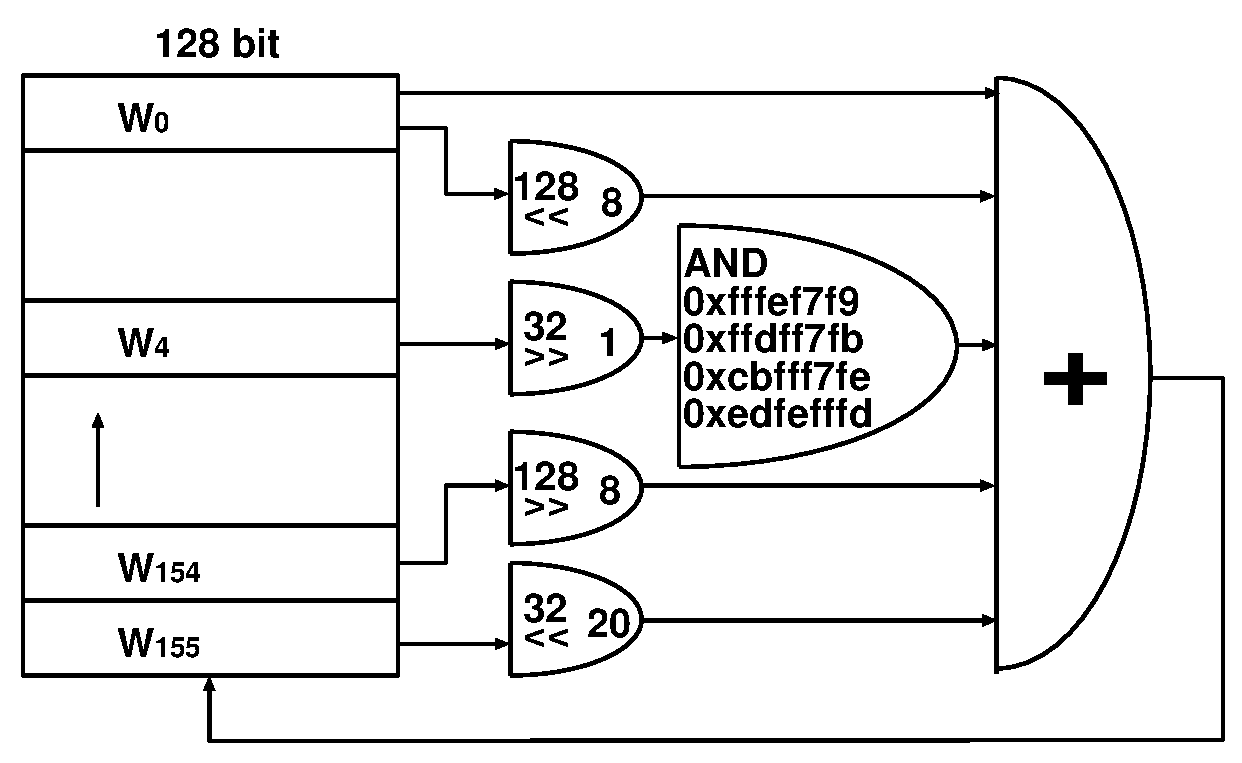
\includegraphics[width=0.7\linewidth]{sfmt-b2.eps}
\end{center}
\caption{A circuit-like description of SFMT19937.}
\label{fig:SFMT-B2}
\end{figure}

\subsection{How we selected the recursion and parameters.}
SFMT19937 is a 128-bit integer generator, but 
we may regard it as a 32-bit (64-bit) integer generator, by
partitioning each 128-bit into four 32-bit (two 64-bit, respectively)
integers. 
Let $\bx$ be a 128-bit integer. Then we denote
by 
$\bx[0]$ the 32 LSBs of $\bx$, 
$\bx[1]$ the 33rd--64th bits,
$\bx[2]$ the 65rd--96th bits,
and $\bx[3]$ the 32 MSBs. Thus, $\bx$ is
the concatenation of 
$\bx[3], \bx[2], \bx[1], \bx[0]$, in this order.

SFMT generates a sequence
$\bx_0, \bx_1, \bx_2, \ldots$ of 128-bit integers. 
Then, they are converted to a sequence of 32-bit integers
$\bx_0[0], \bx_0[1], \bx_0[2], \bx_0[3], \bx_1[0], \bx_1[1],\ldots$,
or a sequence of 64-bit integers
$\bx_0[1]\bx_0[0], \bx_0[3]\bx_0[2], \bx_1[1]\bx_1[0]$,
i.e., by the so-called little-endian system.

We write codes to compute (the lower bounds of) the period
(see \S\ref{sec:period}),
the dimension of equidistribution (DE, see below),
and to measure the generation speed for Pentium SSE2
and PowerPC altivec, with and without SIMD, as 32-bit 
or 64-bit integer generators. 

We fix a type of recursion,
then using a small model (e.g. the period is a smaller
Mersenne prime $2^{607}-1$), we tested whether it
attains the desired period, good DE, and fast generations,
by try-and-errors.

Then, we searched for the parameters 
with period being a nonzero multiple of $2^{19937}-1$. 
Roughly 10 sets of parameters are found per a day,
by using four AMD Athlon 64 machines. 
We selected the best parameter with respect to DE.

We briefly recall the definition of dimension of 
equidistribution (cf. \cite{CLT}). 
\begin{definition}\label{def:DE}
A periodic sequence with period $P$
$$\chi:=\bx_0, \bx_1, \ldots, \bx_{P-1}, \bx_P=\bx_0, \ldots$$
of $v$-bit integers is said to be {\em $k$-dimensionally equidistributed}
if any $kv$-bit pattern occurs equally often as a $k$-tuple
$$
(\bx_i, \bx_{i+1}, \ldots, \bx_{i+k-1})
$$
for a period $i=0,\ldots, P-1$.
We allow an exception for 
the all-zero pattern, which may occur once less often.
The largest value of such $k$ is called the dimension 
of equidistribution (DE).
\end{definition}
This last loosening of the condition is practically 
necessary, because the zero state does not occur
in an $\F2$-linear generator. 

We want to generalize this definition slightly.
We define the $k$-window set of the periodic sequence $\chi$
as
$$
W_k(\chi):=
\{(\bx_i, \bx_{i+1}, \ldots, \bx_{i+k-1}) | 
i =0,1,\ldots, P-1\},
$$
which is considered as a {\em multi-set}, namely, 
the multiplicity of each element is considered. 

For a non-negative integer $m$ and a multi-set $T$,
let us denote by $m \cdot T$ the multi-set 
where the multiplicity of each element in $T$ is
multiplied by $m$. Then, the above definition of
equidistribution is equivalent to 
$$
W_k(\chi)=(m\cdot O^k) \setminus \{{\mathbf 0}\},
$$
where $m$ is the multiplicity of the occurrences,
and the operator $\setminus$ means that the multiplicity
of ${\mathbf 0}$ is subtracted by one. 

\begin{definition}
In the above setting, if there exists an integer $m$ 
and a multi-subset
$D \subset (m\cdot O^k)$
such that
$$
W_k(\chi)=(m\cdot O^k) \setminus D,
$$
we say that $\chi$ is $k$-dimensionally equidistributed 
with defect ratio $\#(D)/\#(m \cdot O^k)$, 
where the cardinality is counted with multiplicity. 
\end{definition}
Thus, in Definition~\ref{def:DE}, the defect ratio upto $1/(P+1)$
is allowed to claim the dimension of equidistribution. 
In the following, the dimension of equidistribution 
allows the defect ratio upto $2^{-19937}$. 

For a $w$-bit integer sequence, its {\em dimension of 
equidistribution at $v$-bit accuracy} $k(v)$
is defined as the DE of the $v$-bit sequence, obtained by extracting
the $v$ MSBs from each of $w$-bit integers.
There is an upper bound 
$$
k(v) \leq \lfloor \log_2 (P+1) / v \rfloor.
$$
The gap of realized $k(v)$ from the upperbound is
called the dimension defect at $v$ of the sequence,
and denoted by
$$
d(v):=\lfloor \log_2 (P+1) / v \rfloor -k(v).
$$
The summation of all the dimension defects at
$1 \leq v \leq 32$ is called the total dimension defect, 
denoted by $\Delta$.

There is a difficulty in computing $k(v)$ when 
a 128-bit integer generator is used as a 32-bit 
(or 64-bit) integer generator.
We solved this by using weighted lattice method,
generalizing \cite{CLT}. Since the algorithm involves
rather complicated mathematics, we omit it here
(we are preparing another article for this). 

The algorithm gives a (rather tight) 
lower bound $k'(v)$ of $k(v)$ for each $v$, 
and $k'(v) \leq \lceil 19937/v \rceil$ holds
for SFMT19937.
Consequently, we redefine the dimension defect for SFMT19937 by
$$
d(v):=\lceil 19937/v \rceil - k'(v) 
\mbox{ and } \Delta:=\sum_{v=1}^w d(v).
$$

\section{Comparison of the speed}\label{sec:comp-speed}
We compared two algorithms: MT19937 and SFMT19937,
with implementations with and without SIMD instructions.

We measured the speeds for four different CPUs:
Pentium M 1.4GHz, IV 3GHz, 
Athlon 64 3800+, and Power PC G4 1.33GHz.  
In returning the random values, we use two different ways.
One is the sequencial generation, where one 32-bit random 
integer is returned for one call. This is disadvantageous for 
SFMT, since it requires partitioning of a 128-bit integer
into 32-bit integers.

The other is the block generation, where an array
of random integers is generated for one call (for 
detail, see \S\ref{sec:block} below). 
We measured the consumed CPU time in second, 
for approximately $10^8$ generations. More precisely,
in the block generation case, we generate $624 \times 128$
of 32-bit random integers by one call, and it is iterated
for 1252 times. This amounts to generating
$99999744\sim 10^8$ of 32-bit integers. 
In the sequential generation case, the same number 
of 32-bit integers are generated, one per a call.
To avoid the function call, the code is written 
in C++ and inline expansion is specified.

Table~\ref{tab:speed} summarizes the comparison of 
the speed. The first four lines list the CPU-time
(in second) needed to generate (roughly) $10^8$ of
32-bit integers, for Pentium-M CPU with intel C/C++
compiler. The first line lists the seconds for
block-generation scheme. The second line shows the 
ratio of the seconds, where the base is taken at 
SFMT(SIMD). Thus, SFMT coded in SIMD is 1.87 times
faster than MT coded in SIMD, and 3.53 times faster
than MT without SIMD. The third line lists the seconds
for sequential generation scheme. The fourth line
lists the ratio of them, with the basis taken
at SFMT(SIMD) block-generation (not sequential). 
Thus, the block-generation of SFMT(SIMD) is 3.03 times
faster than the sequential-generation of SFMT(SIMD).

Roughly saying, in the block generation, 
SFMT(SIMD) is twice faster than MT(SIMD),
and four times faster than MT without using SIMD.
Even in the sequential generation case
where SFMT is
disadvantageous,
still SFMT(SIMD) is considerably faster than MT(SIMD).

\begin{table}
\begin{center}
\begin{tabular}{|c|c||c|c|c|c|}
\hline
CPU/compiler & return & MT & MT(SIMD) & SFMT & SFMT(SIMD)  \\ \hline \hline
Pentium-M  & block   & 0.903 & 0.479 & 0.584 &0.256  \\ 
\cline{3-6}
 1.4GHz, & (ratio) & 3.53\phantom{0}  & 1.87\phantom{0}  & 2.28\phantom{0}  & 1.00\phantom{0}\\ 
\cline{2-6}
 intel C/C++ &  seq     & 1.112 & 1.016 & 1.007 & 0.776 \\ 
\cline{3-6}
 ver. 9.0 & (ratio) & 4.34\phantom{0} & 3.97\phantom{0}  & 3.93\phantom{0}  & 3.03\phantom{0} \\ 
\hline
 Pentium-IV & block & 0.498 & 0.300 & 0.387 & 0.175 \\ 
\cline{3-6}
 3GHz, & (ratio)& 2.85\phantom{0} & 1.71\phantom{0}  & 2.21\phantom{0}
  & 1.00\phantom{0}  \\ 
\cline{2-6}
 intel C/C++ & seq   & 0.847 & 0.724 & 0.648 & 0.449 \\
\cline{3-6}
 ver. 9.0 & (ratio)& 4.84\phantom{0} & 4.14\phantom{0}  & 3.70\phantom{0}
  & 2.57\phantom{0}  \\ 
\hline
 Athlon 64 3800+& block & 0.543 & 0.264 & 0.272 & 0.112 \\
\cline{3-6}
 2.4GHz, & (ratio)& 4.85\phantom{0} & 2.36\phantom{0}  & 2.43\phantom{0} & 1.00\phantom{0} \\ 
\cline{2-6}
 gcc & seq & 0.487 & 0.319 & 0.407 & 0.312  \\ 
\cline{3-6}
 ver. 4.0.2 & (ratio)& 4.35\phantom{0} & 2.85\phantom{0}  & 3.63\phantom{0} & 2.79\phantom{0} \\ 
\hline
Power PC G4 & block & 1.406 & 0.479 & 0.919 & 0.176 \\ 
\cline{3-6}
1.33GHz, & (ratio)& 7.99\phantom{0} & 2.72\phantom{0}  & 5.22\phantom{0} & 1.00\phantom{0}\\ 
\cline{2-6}
 gcc & seq & 0.942 & 0.543 & 0.974 & 0.495 \\ 
\cline{3-6}
 ver.4.0.0 & (ratio)& 5.35\phantom{0} & 3.09\phantom{0} & 5.53\phantom{0} & 2.81\phantom{0} \\ 
\hline
\end{tabular}
\end{center}
\caption{The CPU time (sec.) for $10^8$ generations of 32-bit integers,
for four different CPUs and two different return-value systems. 
The ratio to the SFMT coded in SIMD is listed, too.}\label{tab:speed}
\end{table}

\begin{table}
\begin{center}
\begin{tabular}{|c|c||c|c|c|c|c|c|}
\hline
CPU & return & mrg & rand48 & rand & random256g2 & well & xor3  \\ \hline \hline
Pentium M & block & 3.414  & 1.412  & 0.440  & 0.310  & 2.273  & 0.300 \\
\cline{2-8}
 & seq & 3.425  & 1.252  & 0.691  & 1.002  & 2.834  & 1.221 \\ \hline
Pentium IV & block & 2.546  & 1.249  & 0.406  & 0.109  & 1.218  & 0.313 \\
\cline{2-8}
 & seq & 2.515  & 1.171  & 0.594  & 0.562  & 1.531  & 0.844 \\ \hline
Athlon & block & 2.160  & 1.660  & 0.210  & 0.250  & 0.940  & 0.370 \\
\cline{2-8}
 & seq & 2.090  & 1.490  & 0.200  & 0.210  & 1.100  & 0.500 \\ \hline
PowerPC & block & 2.340  & 1.210  & 0.410  & 0.680  & 1.890  & 0.710 \\
\cline{2-8}
 & seq & 2.250  & 0.820  & 0.370  & 0.990  & 1.910  & 1.010 \\ \hline
\end{tabular}
\end{center}
\caption{The CPU time (sec.) for $10^8$ generations of 32-bit integers,
for four different CPUs and two different return-value systems. 
The ratio to the SFMT coded in SIMD is listed, too.}\label{tab:speed-other}
\end{table}

\section{Dimension of equidistribution}
The total dimension defect $\Delta$ of SFMT19937
is $4188$, which is smaller than $6750$ of MT19937.

Table~\ref{tab:dd} lists the dimension defects $d(v)$
of SFMT19937 (as a 32-bit integer generator) 
and MT19937 for $v=1,2,\ldots, 32$.
SFMT has smaller values of the defect $d(v)$
at 26 values of $v$. The converse holds for 6 values of
$v$, but the difference is small.
\begin{table}
\begin{tabular}{|c|rr||c|rr||c|rr||c|rr|} \hline
$v$ & MT & SFMT & $v$ & MT & SFMT & $v$ & MT & SFMT & $v$ & MT & SFMT\\ \hline
$d(1)$ & 0 & 0 & $d(9)$ & 346 & 1 & $d(17)$ & 549 & 543 & $d(25)$ & 174 & 173 \\
$d(2)$ & 0 & *2 & $d(10)$ & 124 & 0 & $d(18)$ & 484 & 478 & $d(26)$ & 143 & 142
\\
$d(3)$ & 405 & 1 & $d(11)$ & 564 & 0 & $d(19)$ & 426 & 425 & $d(27)$ & 115 & 114
\\
$d(4)$ & 0 & *2 & $d(12)$ & 415 & 117 & $d(20)$ & 373 & 372 & $d(28)$ & 89 & 88
\\
$d(5)$ & 249 & 2 & $d(13)$ & 287 & 285 & $d(21)$ & 326 & 325 & $d(29)$ & 64 & 63
\\
$d(6)$ & 207 & 0 & $d(14)$ & 178 & 176 & $d(22)$ & 283 & 282 & $d(30)$ & 41 & 40
\\
$d(7)$ & 355 & 1 & $d(15)$ & 83 & *85 & $d(23)$ & 243 & 242 & $d(31)$ & 20 & 19 
\\
$d(8)$ & 0 & *1 & $d(16)$ & 0 & *2 & $d(24)$ & 207 & 206 & $d(32)$ & 0 & *1 \\
\hline

\end{tabular}
\caption{Dimension defects 
$d(v)$ of MT19937 and SFMT19937
as a 32-bit integer generator.
The mark * means that MT has a smaller defect than SFMT
at that accuracy.
}\label{tab:dd}
\end{table}

\begin{figure}
\begin{center}
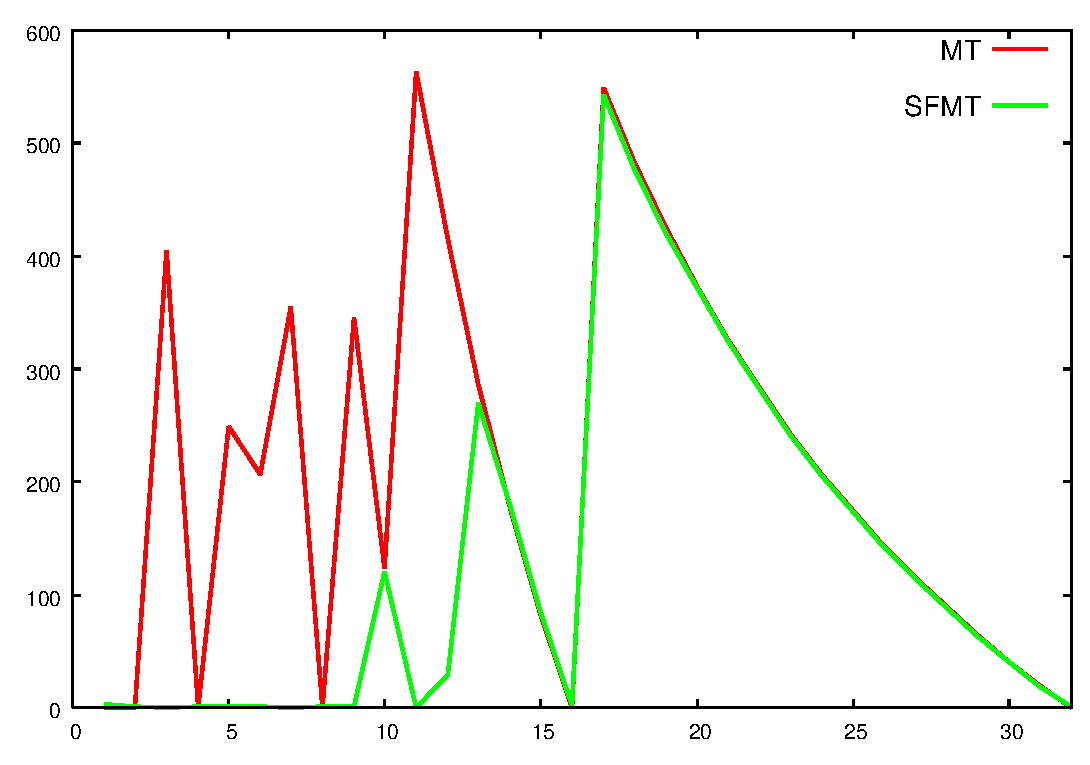
\includegraphics[width=0.8\linewidth,height=0.7\textheight,
keepaspectratio]{delta.eps}
\end{center}
\caption{The dimension defects $d(v)$ of MT (real line) and SFMT (dotted)
for $v=1,2,\ldots, 32$.}
\end{figure}

\section{Concluding remarks}
We proposed SFMT pseudorandom number generators, 
which is a very fast generator with satisfactorily
high dimensional equidistribution property. 

\subsection{Trade-off between the speed and the quality?}
It is difficult to measure the generation speed of a PRNG in a fair way. 
There is an $\F2$-linear generator 
WELL \cite{WELL}, which has the optimal dimension of 
equidistribution (i.e. $\Delta=0$), 
with various periods ($2^{1024}-1$ to $2^{19937}-1$).
If we use the function call to PRNG
for each generation, then not a tiny portion of CPU time
is consumed for hundling the function call, and in the 
experiments in \cite{WELL} or \cite{XORSHIFT}, WELL 
is not so slower than MT. On the other hand, if we avoid
the function call, WELL is much slower than MT as seen
in Table~\ref{tab:speed}. 

Since $\Delta=0$, WELL has a better quality than MT or SFMT
in a theoretical sense. 
However, one may argue on whether this difference is 
observable or not. In the case of $\F2$-linear generator,
the dimension of equidistribution $k(v)$ of $v$-bit accuracy
means that
there is no constant linear relation among the 
$kv$ bits, but there exists a linear relation among
the $(k+1)v$ bits, where $kv$ bits are taken from
all the consequtive $k$ integers ($v$ MSBs of each of them). 
However, the existence of linear relation does not necessarily
mean the existence of the observable bias.
According to \cite{TESTWEIGHT}, it requires $10^{28}$
samples to detect an $\F2$-linear relation with 
15 (or more) terms among 521 bits, by a standard
statistical test. If the number of the 
total bits is increased, 
the necessary sample size is increased. Thus, it seems
that $k(v)$ of SFMT19937 is sufficiently large, far beyond
the level of the observable bias. 
On the other hand, the speed of the generator is 
observable, and important in some purposes. 
Thus, SFMT focuses more on the speed. 

\subsection{Trade-off between the speed and the portability}
There is a trade-off between the speed and the portablity.
We prepare (1) a standard C code of SFMT, which uses 
functions specified in ISO-C only, (2) an optimized C++ code for
Intel Pentium SSE2, and (3) an optimized C++ code for PowerPC. 
The fastest implementation depends on the compiler, its versions and
options. We will put the codes in the homepage {\tt http://www.???}.

\appendix
\section{Computation of  the Period}\label{sec:period}
%\subsection{Reducible transition function}
LFSR may be considered as an automaton, 
with the state space $S=(\F2^{w})^{N}$ 
the state transition function 
$f: S \to S$ given by
$(\bw_0,\ldots,\bw_{N-1})
\mapsto (\bw_1,\ldots,\bw_{N-1}, g(\bw_0,\ldots,\bw_{N-1}))$.  
As a $w$-bit integer generator, the output function is 
$o: S \to \F2^{w},\  (\bw_0,\ldots,\bw_{N-1}) \mapsto \bw_0$.

Let $\chi_f$ be the characteristic polynomial of $f:S \to S$.
If $\chi_f$ is primitive, then the 
period of the state transition takes the maximal value
$2^{\dim(S)}-1$ \cite[\S3.2.2]{knuth:bible}. 
However, to check the primitivity, we need
the integer factorization of this number, which is usually 
impossible for $\dim(S)=nw>10000$. 
On the other hand, the primarity test is much easier than 
the factorization, so many huge primes of the form 
$2^p-1$ are found. 
Such a prime is called a Mersenne prime, and $p$ is
called the Mersenne exponent, which itself is a prime.

MT discards some fixed $r$-bits from the
array $S$, so that $nw-r$ is a Mersenne exponent. 
Then, the primitivity of $\chi_f$ is easily checked
by the algorithm in \cite[\S3.2.2]{knuth:bible}.

Another method is the reducible transition method (RTM), 
which uses a reducible characteristic polynomial.
This is discussed in detail in another article \cite{PMT}, 
so we briefly recall it. 

Let $p$ be the Mersenne exponent, and $N:=\lceil p/w \rceil$.
Then, we randomly choose parameters for the recursion of LFSR
(\ref{eq:recursion}).
By the Berlekamp-Massey Algorithm, 
we compute the minimal polynomial of the (bit) sequence
generated by the linear recursion. By taking the least
common multiple for several initial values, we have the 
minimal polynomial of the transition $f$. With high 
probability its degree coincides with $\dim(S)$, and then
it is the characteristic polynomial $\chi_f$. 
(Note that a direct computation of $\det(tI-f)$ is difficult
 because $\dim(s)>10000$.)

By using a sieve, we remove factors of small degree from $\chi_f$,
until it turns out that it has no irreducible factor of degree $p$,
or it has some factor of degree $p$. In the latter case, it is 
passed to the primitivity test in \cite[\S3.2.2]{knuth:bible}.

Suppose that we found such a recursion. Then, 
we have a factorization
$$
\chi_f=\phi_p \phi_r,
$$
where $\phi_p$ is a primitive polynomial of degree $p$
and $\phi_r$ is a polynomial of degree $r=wN-p$. These are coprime, 
if we assume $p>r$.
By linear algebra, we have a decomposition into $f$-invariant subspaces
$$
S=V_p \oplus V_r,
$$
where $f|_{V_p}$ has the minimal polynomial $\phi_p$
and $f|_{V_r}$ has the characteritic polynomial $\phi_r$.
For any element $s \in S$, we denote $s=s_p+s_r$ for the corresponding
decomposition. 

The period length of the state transition is the least common multiple
of that started from $s_p$ and that started from $s_r$. Hence, 
if $s_p \neq 0$, then the period is a nonzero multiple of $2^p-1$. 
Using this method, we checked the following. 
\begin{proposition}
The period of SFMT19937 as 128-bit integer generator is 
a nonzero multiple of $2^{19937}-1$, if $\bw_0$ is set to 
the value ???.
\end{proposition}
The choice of the value for $\bw_0$ is to assure that $s_p\neq 0$.

\section{Block-generation}\label{sec:block}
In the block-generation scheme, 
the user of PRNG specifies an array
of 32-bit (64-bit) integers of the length
a multiple of 624 (312, respectively).
By calling {\tt fill\_array} function 
with a pointer to this array and the length, 
the PRNG routine fills up this array with
pseudorandom integers. SFMT19937 keeps the state
space in an internal array of 128-bit integers of length 156,
and then generate 156 integers in the user-specified 
array by the recursion (\ref{eq:rec-SFMT}). 
Then, using a part of the user-specified array as a 
state space, SFMT19937 generates and fills up the array
by the same recursion. After filling up, the last
156 of 128-bit integers are copied to the internal array
of SFMT19937. Figure~\ref{fig:B1} describes this scheme.
This makes the generation much faster.

\begin{figure}
\begin{center}
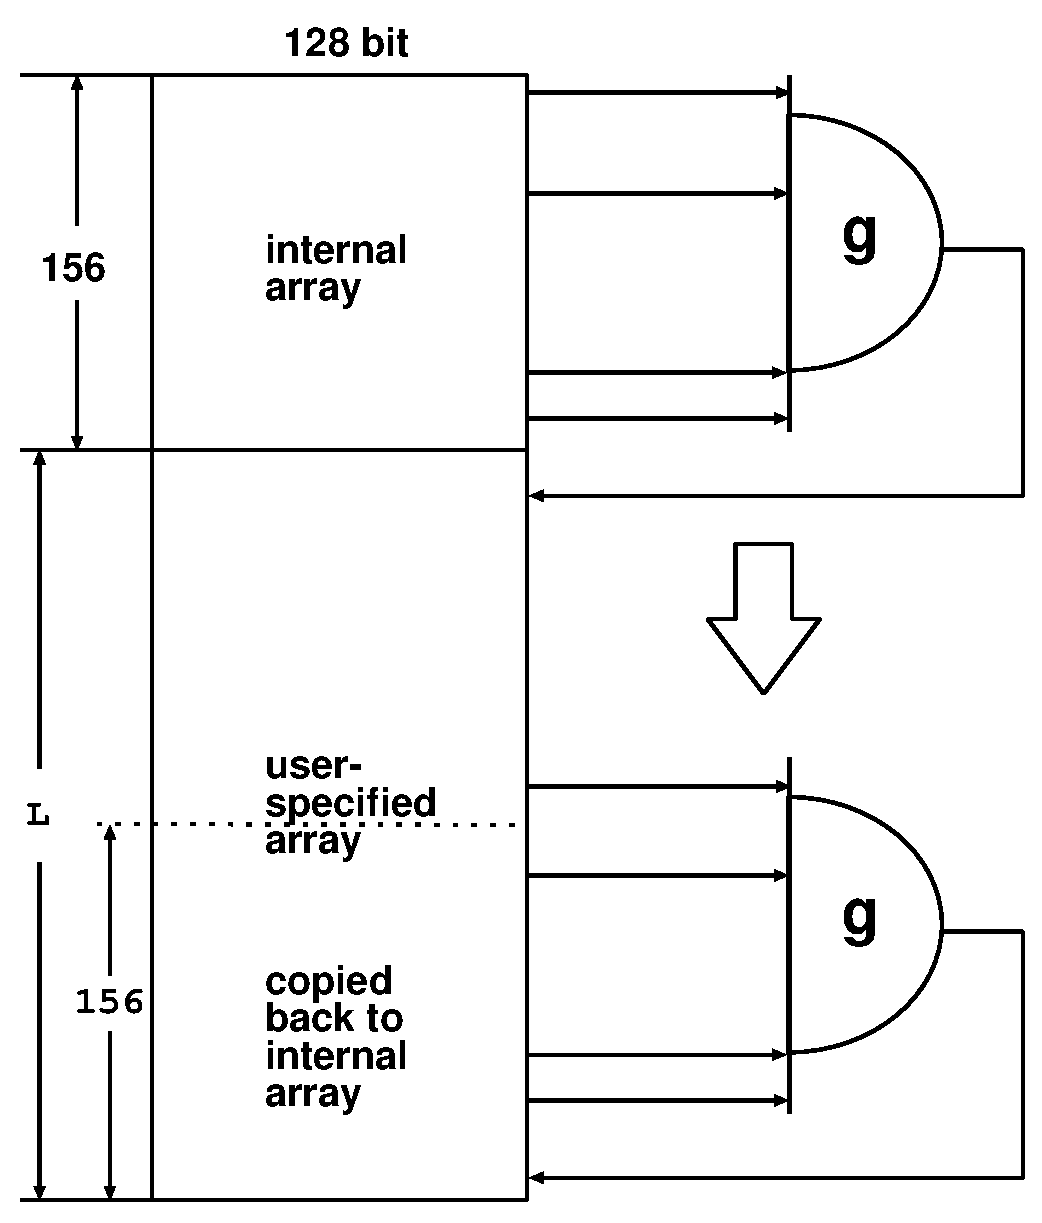
\includegraphics[width=0.7\linewidth,height=0.7\textheight,
keepaspectratio]{fill_array.eps}
\end{center}
\caption{Block-generation scheme}
\label{fig:B1}
\end{figure}

\bibliographystyle{acmtrans}
\bibliography{kuramoto}
\begin{received}
\end{received}
\end{document}
